%\begin{frame}
%    \centering
%    \textbf{\Large{Multiwavelet Linear Response}}
%\end{frame}

\begin{frame}
    \frametitle{Integral formulation linear response}
    \centering
    \textbf{The Sternheimer equations (coupled-perturbed HF/KS)}
    \begin{equation}
        \nonumber
        \hat{F}^{(0)}\ket{\orbital_i^{(1)}} + \hat{F}^{(1)}\ket{\orbital_i^{(0)}} = 
        \sum_jF_{ij}^{(0)}\ket{\orbital_j^{(1)}} + \sum_j F_{ij}^{(1)}\ket{\orbital_j^{(0)}}
    \end{equation}

    \vspace{10mm}

    \textbf{are solved in the same way as the ground state}
    \begin{align}
        \nonumber
        \ket{\orbital_i^{(1)}} =\
        -2\Helmholtz{\hat{V}^{(0)}\ket{\orbital_i^{(1)}}
        + \left(1 - \hat{\rho}^{(0)}\right)\hat{F}^{(1)}\ket{\orbital_i^{(0)}}}
    \end{align}

\vspace{5mm}
\centering
\tiny
T. Yanai \etal,
{\it Mol. Phys.},
\textbf{103:2-3} 
(2005)\\
H. Sekino \etal,
{\it J. Chem. Phys.},
\textbf{129} 
(2008)\\
T. Yanai, \etal,
\it{Phys. Chem. Chem. Phys.}, 
\textbf{17}
(2015)

\end{frame}

%\begin{frame}
%\frametitle{Integral formulation linear response}
%
%\begin{columns}
%\begin{column}[b]{0.48\linewidth}
%\centering
%\textbf{Time-dependent perturbation}
%\begin{align}
%    \nonumber
%    \hat{H}^{(1)}(t) &= 
%    \hat{h}^{(1)}e^{i\omega t} +
%    \hat{h}^{(1)\dag}e^{-i\omega t}\\
%    \nonumber
%    &\ \\
%    \nonumber
%    \rho^{(1)}(t) &= 
%    \tilde{\rho}^{(1)}e^{i\omega t} +
%    \tilde{\rho}^{(1)\dag}e^{-i\omega t}\\
%    \nonumber
%    &\ \\
%    \nonumber
%    \pert{\tilde{\rho}}{1}(r,r') &= 
%    \sum_i x_i(r)\orbital_i^\dag(r') + \orbital_i(r)y_i^\dag(r')
%\end{align}
%\end{column}
%
%\begin{column}[b]{0.48\linewidth}
%\centering
%\textbf{First-order operators}
%\begin{align}
%    \nonumber
%    \pert{\coulomb}{1} \orbital_p &=
%        \int\frac{\pert{\tilde{\rho}}{1}(r',r')\orbital_p(r)}{|r-r'|} \ud r' \\
%    \nonumber
%    \pert{\exchange}{1} \orbital_p &=
%        \int\frac{\pert{\tilde{\rho}}{1}(r,r')\orbital_p(r')}{|r-r'|} \ud r' \\
%    \nonumber
%    \pert{\xc}{1} \orbital_p &= 
%        \bigg[\frac{\delta^2 E_{xc}}{\delta \rho^2}
%        \big[\pert{\rho}{0}\big]*\pert{\tilde{\rho}}{1}\bigg] \orbital_p
%\end{align}
%\end{column}
%\end{columns}
%
%\vspace{7mm}
%\centering
%\textbf{Working equations for dynamic linear response}
%\begin{align}
%    \nonumber
%    x_i &= -2 \Helmholtzp{
%    \pert{\potential}{0}x_i +
%    \Big(1 - \pert{\density}{0}\Big)
%    \Big(\pert{\hamiltonian}{1} + \pert{\potential}{1}\Big)\orbital_i}\\
%    \nonumber
%    y_i &= -2 \Helmholtzm{
%    \pert{\potential}{0}y_i +
%    \Big(1 - \pert{\density}{0}\Big)
%    \Big(\pert{\hamiltonian}{1} + \pert{\potential}{1}\Big)^\dag\orbital_i}
%\end{align}
%
%
%\vspace{7mm}
%
%\begin{columns}
%\begin{column}[b]{0.48\linewidth}
%\centering
%\textbf{BSH operators} 
%\begin{equation}
%    \nonumber
%    2\hat{G}_i^{(\pm)} = \Big[\hat{T} - (\epsilon_i \pm \omega)\Big]^{-1} 
%\end{equation}
%\end{column}
%
%\begin{column}[b]{0.48\linewidth}
%\centering
%\textbf{Density operator}
%\begin{equation}
%    \nonumber
%    \pert{\density}{0} = \sum_i \ket{\orbital_i}\bra{\orbital_i}
%\end{equation}
%\end{column}
%\end{columns}
%
%\vspace{5mm}
%\centering
%\tiny
%T. Yanai \etal,
%{\it Mol. Phys.},
%\textbf{103:2-3} 
%(2005)\\
%H. Sekino \etal,
%{\it J. Chem. Phys.},
%\textbf{129} 
%(2008)\\
%T. Yanai, \etal,
%\it{Phys. Chem. Chem. Phys.}, 
%\textbf{(published online)},
%(2015)
%
%\end{frame}

%\begin{frame}
%\frametitle{Polarizability}
%\begin{columns}
%
%\begin{column}[b]{0.3\textwidth}
%\centering
%\textbf{Electric dipole operator}
%\begin{equation}
%    \nonumber
%    \pert{\hamiltonian}{E} = \boldsymbol{r}_O
%\end{equation}
%\end{column}
%
%
%\begin{column}[b]{0.7\textwidth}
%\centering
%\textbf{Polarizability}
%\begin{equation}
%    \nonumber
%    \alpha 
%    %= \int \pert{\hamiltonian}{E} \ \pert{\rho}{E} \ dr
%    = \sum_i 
%    \bra{\orbital_i}\pert{\hamiltonian}{E} \ket{\pert{x_i}{E}} + 
%    \bra{\pert{y_i}{E}}\pert{\hamiltonian}{E}\ket{\orbital_i}
%\end{equation}
%\end{column}
%\end{columns}
%
%\vspace{5mm}
%
%
%\begin{table}
%%\tiny
%\begin{tabular}{r|c|cr|cr}
%\multicolumn{6}{c}{\textbf{LDA polarizability of methyloxirane (a.u.)}}\\
%\hline
%\hline
%	             &               &               &               &               &               \\
%                     & $E^{tot}$     & Static        &Time           & Dynamic       &Time           \\
%    \hspace{20mm}\   &\hspace{20mm}\ &\hspace{20mm}\ &\hspace{05mm}\ &\hspace{20mm}\ &\hspace{05mm}\ \\
%    MRChem $10^{-2}$ & -191.5975     & 44.0764       &   30m         & 45.2747       &   1h          \\
%    MRChem $10^{-3}$ & -191.5622     & 44.0939       &    1h         & 45.2907       &   2h          \\
%    MRChem $10^{-4}$ & -191.5619     & 44.0935       &    2h         & 45.2903       &   3h          \\
%	             &               &               &               &               &               \\
%    aug-cc-pVQZ      & -191.5563     & 44.1326       &    1h         & 45.3380       &   2h          \\
%	cc-pVQZ      & -191.5549     & 42.3602       &   30m         & 43.4064       &   1h          \\
%    aug-cc-pVDZ      & -191.4817     & 44.0050       &    1m         & 45.2025       &   2m          \\
%	cc-pVDZ      & -191.4622     & 36.5586       &    $<$1m      & 37.3993       &   1m          \\
%	             &               &               &               &               &               \\
%\hline
%\hline
%\end{tabular}
%\end{table}
%
%\centering
%\scriptsize
%\it{Wall time given on 16 CPUs}\\
%\it{GTO calculations using Dalton}\\
%\it{Dynamic response at sodium D line (589.3 nm) wavelength}
%
%\end{frame}


%\begin{frame}
%\frametitle{Magnetizability}
%\begin{columns}
%
%\begin{column}[b]{0.5\textwidth}
%\centering
%\textbf{Diamagnetic magnetizability}
%\begin{equation}
%    \nonumber
%    \pert{\hamiltonian}{B,B} = 
%    -\frac{1}{4}\Big(r_O^2\boldsymbol{I} 
%    -\boldsymbol{r}_O\boldsymbol{r}_O^T\Big)
%\end{equation}
%
%\vspace{2mm}
%
%\begin{align}
%    \nonumber
%    \chi^{dia} &= \sum_i \bra{\orbital_i} \pert{\hamiltonian}{B,B} \ket{\orbital_i}
%%    \nonumber
%%    \chi^{dia} &= \int \pert{\hat{h}}{dia} \rho \ud r
%\end{align}
%\end{column}
%
%\begin{column}[b]{0.5\textwidth}
%\centering
%\textbf{Paramagnetic magnetizability}
%\begin{equation}
%    \nonumber
%    \pert{\hamiltonian}{B} = -i \boldsymbol{r}_O\times\nabla
%\end{equation}
%\vspace{2mm}
%\begin{align}
%    \nonumber
%    \chi^{para} &= \sum_i 
%    \bra{\orbital_i}\pert{\hamiltonian}{B} \ket{\pert{x_i}{B}} + 
%    \bra{\pert{y_i}{B}}\pert{\hamiltonian}{B}\ket{\orbital_i}
%%    \nonumber
%%    \chi^{para} &= \int \pert{\hat{h}}{orb}\pert{\tilde{\rho}}{orb} \ud r
%\end{align}
%\end{column}
%
%\end{columns}
%\vspace{6mm}
%
%\begin{table}
%%\tiny
%\centering
%\begin{tabular}{r|c|crrr}
%\multicolumn{6}{c}{\textbf{Hartree-Fock magnetizability of methyloxirane (a.u.)}}\\
%\hline
%\hline
%                     &               &               &                     &                     &               \\
%                     &$E^{tot}$      & GIAO          & $O=(0,0,0)$         & $O=(5,5,5)$         &Time           \\
%    \hspace{15mm}\   &\hspace{15mm}\ &\hspace{15mm}\ &\hspace{15mm}\       &\hspace{15mm}\       &\hspace{05mm}\ \\
%    MRChem $10^{-2}$ & -192.0425     &               &  -9.5497\ \ \ \ \ \ &  -9.9222\ \ \ \ \ \ &    4h         \\
%    MRChem $10^{-3}$ & -192.0002     &               &  -9.4730\ \ \ \ \ \ &  -9.4363\ \ \ \ \ \ &    6h         \\
%    MRChem $10^{-4}$ & -192.0000     &               &  -9.4758\ \ \ \ \ \ &  -9.4795\ \ \ \ \ \ &   12h         \\
%                     &               &               &                     &                     &               \\
%    aug-cc-pVQZ      & -191.9968     & -9.4736       & -10.5253\ \ \ \ \ \ & -26.0533\ \ \ \ \ \ &    2h         \\
%	cc-pVQZ      & -191.9960     & -9.4681       & -10.8019\ \ \ \ \ \ & -29.2395\ \ \ \ \ \ &    1h         \\
%    aug-cc-pVDZ      & -191.9357     & -9.5369       & -15.4438\ \ \ \ \ \ &-101.6430\ \ \ \ \ \ &    1m         \\
%	cc-pVDZ      & -191.9232     & -9.4924       & -19.0342\ \ \ \ \ \ &-140.0203\ \ \ \ \ \ &    $<$1m      \\
%                     &               &               &                     &                     &               \\
%\hline
%\hline
%\end{tabular}
%\end{table}
%
%\centering
%\scriptsize
%\it{Wall time given on 16 CPUs}\\
%\it{GTO calculations using Dalton}
%
%\end{frame}
%
%
%\begin{frame}
%\frametitle{Nuclear shielding}
%\begin{columns}
%
%\begin{column}[b]{0.4\textwidth}
%\centering
%\textbf{Diamagnetic shielding}
%\begin{equation}
%    \nonumber
%    \pert{\hamiltonian}{M_K,B} =
%    \frac{\alpha}{2}\frac{\Big(r_O^Tr_K\boldsymbol{I} - 
%    \boldsymbol{r}_O\boldsymbol{r}_O^T\Big)}{r_K^3}
%\end{equation}
%\vspace{2mm}
%\begin{equation}
%    \nonumber
%    \xi^{dia} = \sum_i \bra{\orbital_i} \pert{\hamiltonian}{M_K,B} \ket{\orbital_i}
%\end{equation}
%\end{column}
%
%\begin{column}[b]{0.6\textwidth}
%\centering
%\textbf{Paramagnetic shielding}
%\begin{equation}
%    \nonumber
%    \pert{\hamiltonian}{M_K} 
%    = -i \alpha^2 \frac{\boldsymbol{r}_K\times\nabla}{r_K^3} \qquad \qquad
%    \pert{\hamiltonian}{B} = -i \boldsymbol{r}_O\times\nabla
%\end{equation}
%\vspace{2mm}
%\begin{equation}
%    \nonumber
%    \xi^{para} = \sum_i 
%    \bra{\orbital_i}\pert{\hamiltonian}{M_K} \ket{\pert{x_i}{B}} + 
%    \bra{\pert{y_i}{B}}\pert{\hamiltonian}{M_K}\ket{\orbital_i}
%\end{equation}
%\end{column}
%
%\end{columns}
%\vspace{5mm}
%
%\begin{table}
%\tiny
%\centering
%\begin{tabular}{r|c|cccr}
%\multicolumn{6}{c}{\textbf{Hartree-Fock shielding tensor of oxygen in methyloxirane (ppm)}}\\
%\hline
%\hline
%                     &               &               &               &               &               \\
%                     & $E^{tot}$     &$\xi^{dia}$    & $\xi^{para}$  &$\xi^{tot}$    &Time           \\
%       	             &\hspace{15mm}\ &\hspace{15mm}\ &\hspace{15mm}\ &\hspace{15mm}\ &\hspace{05mm}\ \\
%    MRChem $10^{-2}$ & -192.0425     &  446.7869     &  -96.6166     &  350.1703     &    4h         \\
%    MRChem $10^{-3}$ & -192.0002     &  447.3444     &  -91.7855     &  355.5589     &    6h         \\
%    MRChem $10^{-4}$ & -192.0000     &  447.3089     &  -90.9386     &  356.3704     &   12h         \\
%	             &               &               &               &               &               \\
%    aug-cc-pVQZ      & -191.9968     &  447.7508     &  -90.6691     &  357.0817     &    2h         \\
%	cc-pVQZ      & -191.9960     &  447.7833     &  -89.6304     &  358.1529     &    1h         \\
%    aug-cc-pVDZ      & -191.9357     &  451.0119     &  -88.5778     &  362.4341     &    1m         \\
%	cc-pVDZ      & -191.9232     &  451.6103     &  -87.4153     &  364.1950     &    $<$1m      \\
%	             &               &               &               &               &               \\
%\hline
%\hline
%\end{tabular}
%\end{table}
%
%\centering
%\scriptsize
%\it{Wall time given on 16 CPUs}\\
%\it{GTO (GIAOs) calculations using Dalton}
%
%\end{frame}
%
%
%\begin{frame}
%\frametitle{Optical rotation}
%\begin{columns}
%
%\begin{column}[b]{0.5\textwidth}
%\centering
%\textbf{Electric-magnetic polarizability}
%\begin{equation}
%    \nonumber
%    \pert{\hamiltonian}{E} = \boldsymbol{r}_O \qquad \qquad
%    \pert{\hamiltonian}{B} = -i \boldsymbol{r}_O\times\nabla
%\end{equation}
%\vspace{4mm}
%\begin{equation}
%    \nonumber
%    G = \sum_i 
%    \bra{\orbital_i}\pert{\hamiltonian}{B} \ket{\pert{x_i}{E}} + 
%    \bra{\pert{y_i}{E}}\pert{\hamiltonian}{B}\ket{\orbital_i}
%\end{equation}
%\end{column}
%
%\begin{column}[b]{0.5\textwidth}
%\centering
%\textbf{Optical rotation}
%\vspace{2mm}
%\begin{equation}
%    \nonumber
%    \beta = \omega^{-1}Tr\big[G\big]
%\end{equation}
%\vspace{2mm}
%\begin{equation}
%    \nonumber
%    \alpha = \frac{28800\pi^2N_A\nu^2}{c^2M}\beta
%\end{equation}
%\end{column}
%
%\end{columns}
%\vspace{5mm}
%
%\begin{table}
%%\tiny
%\centering
%\begin{tabular}{r|c|rrr}
%\multicolumn{5}{c}{\textbf{LDA optical rotation of methyloxirane (a.u.)}}\\
%\hline
%\hline
%	             &               &                       &                           &               \\
%                     &$E^{tot}$      
%                     &\multicolumn{1}{c}{$\beta$}
%                     &\multicolumn{1}{c}{$\alpha$}
%                     &Time           \\
%    \hspace{20mm}\   &\hspace{20mm}\ &\hspace{20mm}\         &\hspace{20mm}\             &\hspace{5mm}\ \\
%    MRChem $10^{-2}$ & -191.5975     & 0.121265\ \ \ \ \ \ \ &   6.2440\ \ \ \ \ \ \ \ \ &    1h         \\
%    MRChem $10^{-3}$ & -191.5622     & 0.134859\ \ \ \ \ \ \ &   6.9439\ \ \ \ \ \ \ \ \ &    2h         \\
%    MRChem $10^{-4}$ & -191.5619     & 0.136527\ \ \ \ \ \ \ &   7.0298\ \ \ \ \ \ \ \ \ &    3h         \\
%	             &               &                       &                           &               \\
%    aug-cc-pVQZ      & -191.5563     & 0.127538\ \ \ \ \ \ \ &   6.5669\ \ \ \ \ \ \ \ \ &    2h         \\
%	cc-pVQZ      & -191.5549     & 0.016025\ \ \ \ \ \ \ &   0.8249\ \ \ \ \ \ \ \ \ &    1h         \\
%    aug-cc-pVDZ      & -191.4817     & 0.010036\ \ \ \ \ \ \ &   0.5170\ \ \ \ \ \ \ \ \ &    2m         \\
%	cc-pVDZ      & -191.4622     &-0.852053\ \ \ \ \ \ \ & -43.8711\ \ \ \ \ \ \ \ \ &    1m         \\
%	             &               &                       &                           &               \\
%\hline
%\hline
%\end{tabular}
%\end{table}
%
%\centering
%\scriptsize
%\it{Wall time given on 16 CPUs}\\
%\it{GTO (GIAOs) calculations using Dalton}\\
%\it{Dynamic response at sodium D line (589.3 nm) wavelength}
%
%\end{frame}
%
%\begin{frame}
%    \frametitle{Convergence}
%    \begin{center}
%	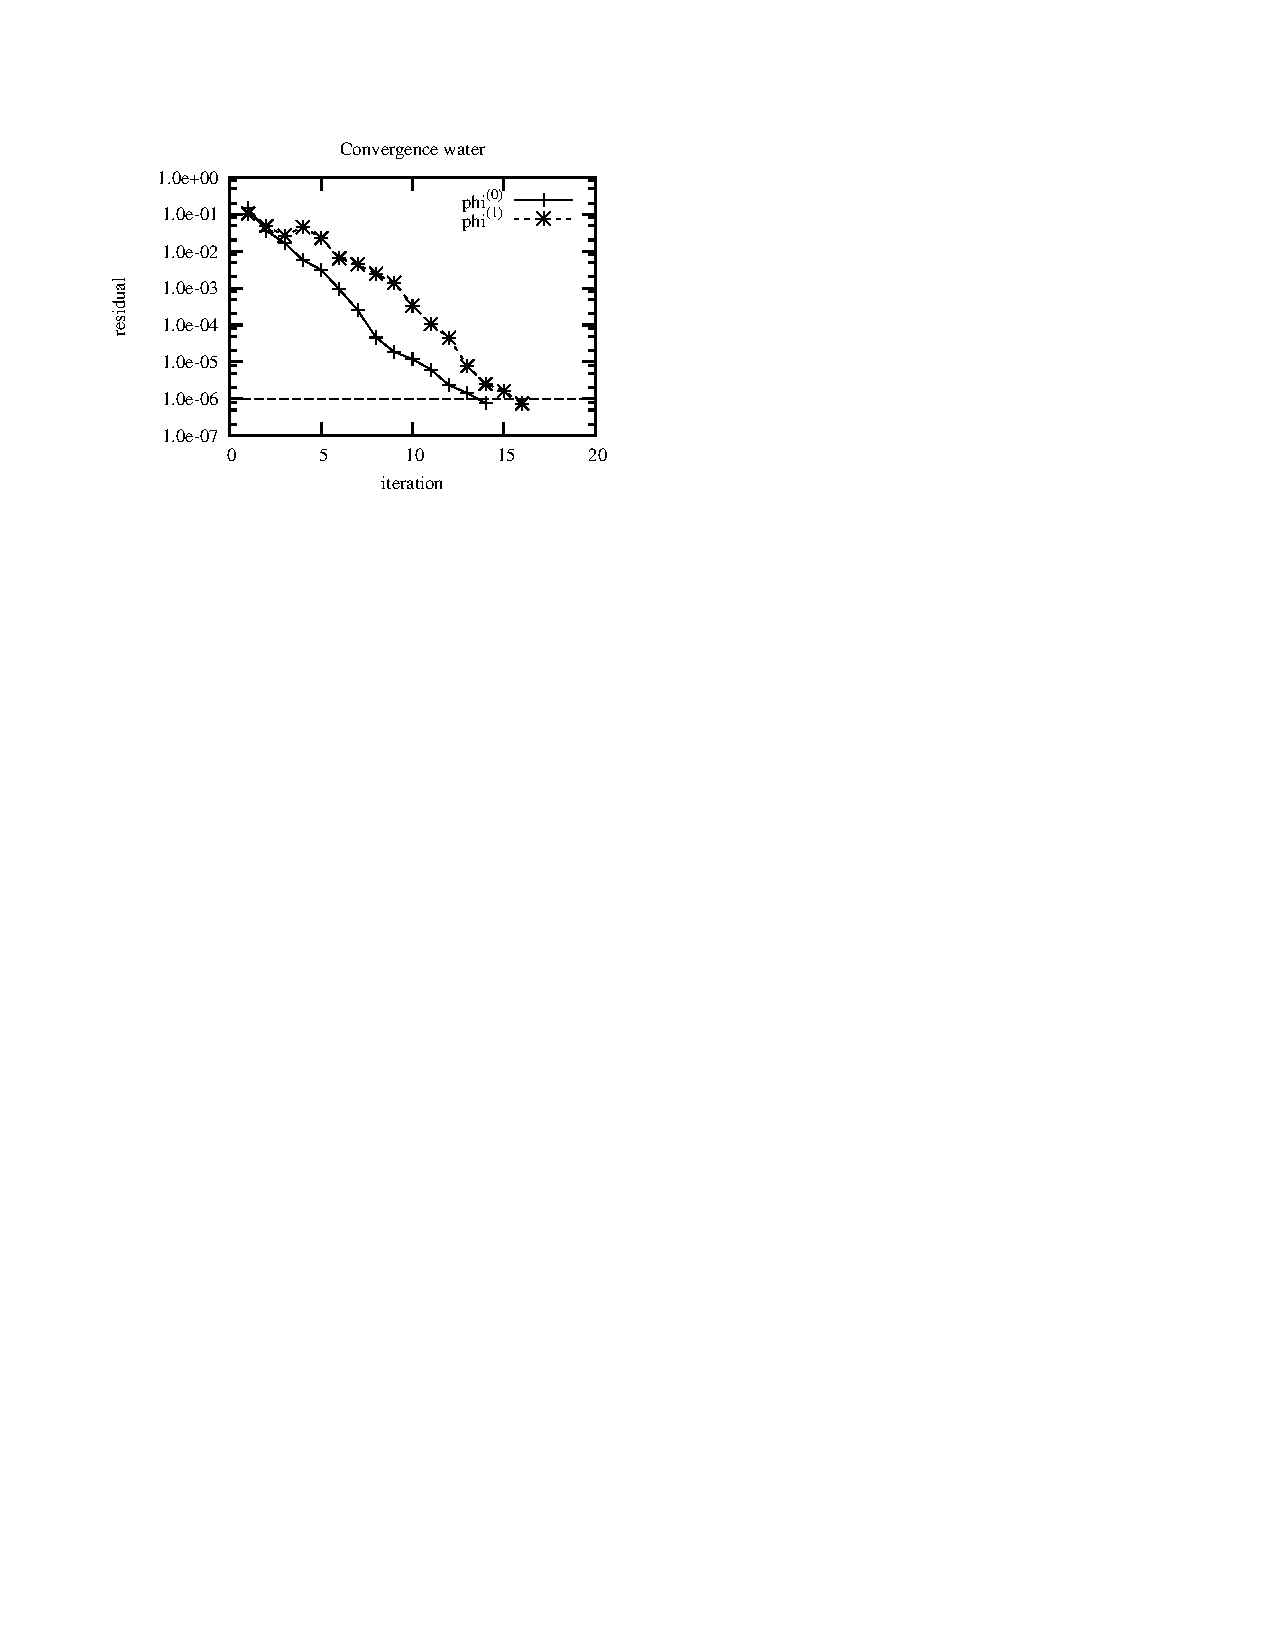
\includegraphics[scale=1.0, clip, viewport = 50 550 300 730]{figures/response_convergence.pdf}
%    \end{center}
%\end{frame}
